% =====================================================================
% When does multi-agent LLM coordination create value?
% Build with: tectonic (XeTeX) or pdflatex/Overleaf.
% =====================================================================
\documentclass[11pt,a4paper]{article}
% Engine auto-detection: XeTeX/LuaTeX (tectonic, xelatex) uses fontspec;
% pdfLaTeX (the Overleaf default) uses T5 + inputenc. Both render Vietnamese
% diacritics correctly, which the author names and the acknowledgement need.
\usepackage{iftex}
\ifPDFTeX
  \usepackage[T5]{fontenc}
  \usepackage[utf8]{inputenc}
  \usepackage[vietnamese,main=english]{babel}
\else
  \usepackage{fontspec}
  % Load by file name so the tectonic font bundle resolves them
  \setmainfont{texgyretermes}[Extension=.otf, UprightFont=*-regular,
    BoldFont=*-bold, ItalicFont=*-italic, BoldItalicFont=*-bolditalic]
  \setsansfont{texgyreheros}[Extension=.otf, UprightFont=*-regular,
    BoldFont=*-bold, ItalicFont=*-italic, BoldItalicFont=*-bolditalic]
  \setmonofont{texgyrecursor}[Extension=.otf, UprightFont=*-regular,
    BoldFont=*-bold, ItalicFont=*-italic, BoldItalicFont=*-bolditalic]
  \usepackage[vietnamese,main=english]{babel}
\fi
\usepackage{amsmath,amssymb}
\usepackage{array}
\usepackage{booktabs}
\usepackage{multirow}
\usepackage[margin=2.4cm]{geometry}
\usepackage{microtype}
\usepackage{xcolor}
\usepackage{graphicx}
\usepackage{tikz}
\usetikzlibrary{arrows.meta,positioning}
\usepackage[colorlinks=true,linkcolor=blue!60!black,citecolor=blue!60!black,urlcolor=blue!60!black]{hyperref}

\setlength{\emergencystretch}{1.5em}
\newcommand{\mucB}{\textsuperscript{\,(level B)}}
\newcommand{\dceil}{\Delta_{\mathrm{ceil}}}
\newcommand{\dhonest}{\Delta_{\mathrm{real}}}
\newcommand{\CEIL}{\mathrm{CEIL}}
\newcommand{\acc}{\mathrm{acc}}

\title{\bfseries When does multi-agent LLM coordination create value?\\
\large An empirical study under three controls}
\author{Dương Trọng Nguyên \and Trương Đình Đức \and Trần Tùng Dương \and Lê Hoàng Quân}
\date{August 2026}

\begin{document}
% ---------------------------------------------------------------- TITLE PAGE
\begin{titlepage}\centering
{\large\bfseries VNU UNIVERSITY OF ENGINEERING AND TECHNOLOGY\par}
{\large\bfseries AI INSTITUTE\par}
\vspace{6pt}
\rule{0.52\linewidth}{0.4pt}\par
\vspace{24pt}


\includegraphics[width=0.28\linewidth]{figs/logo_uet.png}\par
\vspace{32pt}

% Course title: sans-serif, largest type on the page
{\sffamily\bfseries\fontsize{26}{31}\selectfont NATURAL LANGUAGE PROCESSING\par}
\vspace{24pt}

{\sffamily\bfseries\fontsize{15}{18}\selectfont FINAL PROJECT REPORT\par}
\vspace{16pt}

{\fontsize{13.5}{17}\selectfont When does multi-agent LLM coordination create value?\par}
{\fontsize{13.5}{17}\selectfont An empirical study under three controls\par}
\vspace{42pt}

% Group members: two centred columns, student ID aligned under each name
{\normalsize
\begin{tabular}{@{}>{\centering\arraybackslash}p{0.34\linewidth}
                  >{\centering\arraybackslash}p{0.34\linewidth}@{}}
\textbf{Dương Trọng Nguyên} & \textbf{Trương Đình Đức}\\
24022420 & 24021419\\[10pt]
\textbf{Trần Tùng Dương} & \textbf{Lê Hoàng Quân}\\
24022309 & 24022433\\
\end{tabular}\par}
\vspace{24pt}

{\normalsize\textbf{Course code:} INT3406\par}
\vspace{58pt}
{\bfseries Hanoi, August 2026\par}
\vfill
\end{titlepage}

% ---------------------------------------------------------------- ACKNOWLEDGEMENT PAGE
\newpage
\thispagestyle{empty}
\vspace*{1.5cm}

\begin{center}
  {\LARGE\bfseries ACKNOWLEDGEMENT\par}
  \vspace{10pt}
  \rule{0.3\linewidth}{0.6pt}\par
\end{center}
\vspace{1.2cm}

We would like to express our sincere and deepest thanks to our lecturer, \textbf{Trần Hồng Việt}, who taught the Natural Language Processing course at VNU University of Engineering and Technology.

Over the past semester, his dedicated lectures gave us a firm grounding in the subject and in current approaches to large language models. More than that, he trained us in rigorous scientific thinking, in a critical attitude towards our own results, and in a demanding standard of fairness and discipline when running empirical evaluations.

This report is the product of serious and sustained work by the whole group. To get a clear answer to our research question, we spent a great deal of time discussing the design together, setting up controlled comparison conditions, and going through failure cases one by one. The experimental work ran into more than a few obstacles, both methodological and in the compute available to us, but persistence and a willingness to keep learning let the group carry the project through as fully as it could.

Despite our best efforts, this report certainly still has limitations and shortcomings. We would be very glad to receive further comments and guidance from him, so that we can understand the problem more deeply and continue to improve as we go on with our studies.

We wish him continued good health, happiness, and much success in his teaching and in his research.

\vspace{1.8cm}
\begin{flushright}
\textit{Hanoi, August 2026}\\[6pt]
\textbf{The student group}\\[8pt]
\begin{tabular}{rl}
\textbf{Dương Trọng Nguyên} & --- 24022420\\
\textbf{Trương Đình Đức}    & --- 24021419\\
\textbf{Trần Tùng Dương}    & --- 24022309\\
\textbf{Lê Hoàng Quân}      & --- 24022433
\end{tabular}
\end{flushright}

\vfill
\newpage

\begin{abstract}
Multi-agent LLM systems have drawn growing interest because they let a task be divided across
roles such as planning, solving, verifying, and aggregating, on the expectation that the
resulting pipeline does better than a single model working alone. The value that coordination
itself adds is hard to assess, however. Reported comparisons differ in compute budget, in which
model serves as the control, and in how wide an effect they claim. In this report we build one
experimental framework over reasoning and coding benchmarks and use it to study three questions:
how much each role contributes, what happens when one model's solution is passed to another, and
whether a model can be trained to carry out its assigned role. We find that most of the reported
benefit shrinks or disappears once the comparison is made on equal terms. In particular, an
incorrect solution from a weak model can sharply reduce the accuracy of a strong model that reads
it, while an objective verification signal is more reliable than asking a model to judge its own
output. Taken together, the measurements suggest that multi-agent coordination does not produce a
benefit by default. Whether it helps depends on the capability of the models involved, on how
information is routed between them, and on the mechanism used to select and verify candidate
solutions.
\end{abstract}

% =====================================================================
\section{Introduction}\label{sec:intro}

Does chaining several large language models (LLMs) into a multi-agent system of Planner, Solver, Verifier and Aggregator actually beat a single strong model working alone? The natural intuition says yes: split the task, add cross-checking, catch more errors, get better accuracy. Most recent published work in the area supports that intuition.

One experiment unsettles it. On the MATH dataset, a single Qwen-7B model used as the baseline reaches 46.4\% accuracy. Add to its context a wrong solution to the same problem produced by a weaker model (Qwen-1.5B), and Qwen-7B drops to 19.2\%. The strong model got wrong the very problems it could already solve, only because it saw noise from another agent's incorrect solution
(Figure~\ref{fig:exposure}, details in \S\ref{sec:termL}). When the inserted solution is correct instead, the improvement is modest. Letting models read each other's work cuts both ways, and the negative side is larger than the positive one.

\begin{figure}[!ht]\centering
\begin{tikzpicture}[
  box/.style={draw, rounded corners, align=center, font=\small, inner sep=6pt, minimum width=4.2cm},
  every path/.style={-{Stealth[length=2.6mm]}}]

  % Root node
  \node[box] (q) at (0,0) {MATH problem\\{\footnotesize (stratum: weak model's solution is \textbf{wrong}, $n=261$)}};

  % Branch I
  \node[box] (i) at (-3.6,-2.0) {\textbf{Branch $I$}\\Strong model solves alone};
  \node[box] (ri) at (-3.6,-5.2) {Correct \textbf{46.4\%}};

  % Branch E (split across two boxes)
  \node[box, fill=red!6] (e1) at (3.6,-1.8) {\textbf{Branch $E$} \\Weak model solves};
  \node[box, fill=red!6] (e2) at (3.6,-3.6) {Insert the weak model's wrong solution\\into the strong model's context};
  \node[box, fill=red!6] (re) at (3.6,-5.2) {Correct \textbf{19.2\%}};

  % Connecting edges
  \draw (q) -- (i);
  \draw (q) -- (e1);
  \draw (i) -- (ri);
  \draw (e1) -- (e2);
  \draw (e2) -- (re);

\end{tikzpicture}
\caption{\emph{Artifact-exposure experiment} --- showing the strong model the weak model's solution
(pre-registered design, MATH-500): the two branches differ only in whether the context carries
the weak model's wrong solution. The gap of $-27.2$ points ($p \approx 0$) is the main source of
damage in protocols that have models repair each other's work (\S\ref{sec:termL}).}
\label{fig:exposure}
\end{figure}

The conflict between this experiment and the positive results reported earlier comes from three serious problems in how the benefit is measured:

\paragraph{First, compute budget.} With the same 1.5B model, a four-role pipeline emits 2.9 times (on GSM8K) to
6.6 times (on MATH) as many tokens as a single generation. When the roles use models of different sizes, even
tokens are not priced alike -- a token generated by a 7B model costs roughly 4.7--4.9 times the arithmetic (FLOPs)
of a token from a 1.5B model, because inference cost scales with parameter count \cite{kaplan2020}
(\S\ref{sec:baseline}). Comparing an expensive system against a single model without normalizing both to the same compute budget (FLOPs) yields an unfair verdict on efficiency.

\paragraph{Second, choice of baseline.} Most generate-and-repair work measures improvement against the model being repaired (the weak model). In practice, though, the decision a deployer faces is whether to run the whole multi-agent system or just a single strong model. This survey shows that changing the baseline can reverse the sign of the measured effect entirely (\S\ref{sec:baseline},
\S\ref{sec:synthesis}).

\paragraph{Third, denominator.} On MATH with the 1.5B model, 57\% of problems lie outside anything a candidate-selection mechanism could change. Of these, 32\% are too hard, so every candidate answer is wrong, and 25\% are too easy, so every candidate answer is right. In neither case can an aggregation method improve anything. Averaging over the full dataset dilutes the real improvement signal and risks wrongly rejecting interventions that do work (\S\ref{sec:denominator}). Omitting this control \emph{underestimates} the true effect; omitting the other two \emph{overestimates} it --- the three biases do not point the same way, so all three must be applied together and none substitutes for another.

\paragraph{Contributions.} This survey unifies three research lines into a single measurement frame: decomposing contributions by role, analysing the cost and benefit of routing, and analysing information flow. There are four main contributions:
\begin{enumerate}\itemsep2pt
  \item \textbf{Three controls.} We give empirical evidence that when all three controls (compute budget, choice of baseline, and denominator) are applied together, most of the positive effects of multi-agent coordination shrink or reverse (\S\ref{sec:results}).
  \item \textbf{An artifact-exposure experiment} --- showing the strong model the weak model's solution ---
        with a pre-registered design replicated on two domains (Figure~\ref{fig:exposure}): replicating the experiment on two domains pins the damage in generate-and-repair down to exposure to the weak model's incorrect information, not to seeing a solution as such. Generate-and-repair therefore acts as a conduit for answers rather than as a self-correction mechanism (\S\ref{sec:termL}).
  \item \textbf{Two baselines, two opposite conclusions}: against the weak model, the effect grows with the capability gap almost by definition; against the strong model running alone --- the baseline a deployer actually faces --- the effect shrinks and changes sign. Same system, two baselines, two opposite conclusions; the baseline common in the literature is the inflated one (\S\ref{sec:synthesis}).
  \item \textbf{An upper bound on the value of the verifier}: how much a verifier can contribute is bounded by the distance between the oracle ceiling and majority voting. We find that hard verification signals (running code against tests) can approach that ceiling, while learned signals such as LLM-as-a-judge contribute only a small fraction of it (\S\ref{sec:kappa}).
\end{enumerate}
The results were collected under a reliability protocol that fixes the criteria in advance and discards runs that
fail the validity conditions; the protocol is described in
\S\ref{sec:setup}. Of 32 runs in total, 16 (50\%) were discarded before the results were read. The report uses some notation of its own; Table~\ref{tab:cheatsheet} is the quick reference ---
every symbol is defined in full in \S\ref{sec:framework}--\ref{sec:setup} before it is
used.

\begin{table}[t]\centering\small
\renewcommand{\arraystretch}{1.1}
\begin{tabular}{@{}p{0.25\linewidth}p{0.70\linewidth}@{}}\toprule
\multicolumn{2}{@{}l}{\textbf{Notation quick reference} (details: \S\ref{sec:framework}--\ref{sec:setup})}\\\midrule
$P, S, V, A$ & The four roles: plan -- solve -- verify/repair -- select answer\\
$H$ / $\kappa$ / $D$ & Three questions: headroom / exploitability / damage\\
$W$ / $I$ / $E$ & Weak model / strong model alone / strong model that has seen $W$\\
artifact & The weak model's solution (noise injected into the context)\\
$G, L, R$ & Opportunity ($G$), loss ($L$), rescue ($R$)\\
$\dceil$ & Oracle ceiling $\dceil = G-L+R$\\
$\dhonest$ & Effect as deployed: $\acc(E) - \acc(I)$\\
gap; $g^\ast$ & Accuracy difference (strong $-$ weak); sign-flip point of $\dceil$ ($\approx 0.09$)\\
generation & One full solution sampled from a model; the $k$ generations are independent and equally weighted\\
\texttt{maj@}k; \texttt{oracle@}k & Majority voting; oracle ceiling ($k$ generations)\\
\texttt{exec3} / \texttt{llm3} & Candidate selection by: running tests / LLM self-review\\
\texttt{V\_gain}, \texttt{A\_gain} & Change in accuracy when role $V$ or $A$ is added\\
points; CI & Percentage points ($+14.0$ points $= +0.140$); 95\% confidence interval\\
noise floor & Spread when the same configuration is re-measured (up to 7 points per 100 problems)\\
fold; Level A / B & A disjoint block of 60--100 problems, five in total; 5-fold validation ($t$-test) / single illustrative measurement\\\bottomrule
\end{tabular}
\caption{Quick reference for the notation and terminology used in this report.}
\label{tab:cheatsheet}
\end{table}

% =====================================================================
\section{Related work}\label{sec:related}

\paragraph{Generate then select.} Chain-of-thought prompting \cite{wei2022} set the stage for self-consistency
\cite{wang2023}, in which the system samples several independent solutions and settles the answer by majority
voting --- exactly the \texttt{maj@}$k$ baseline of this survey (defined in \S\ref{sec:setup}). Verifier-based selection then branched in two main directions: scoring the reasoning process step by step \cite{lightman2024} and allocating extra compute at inference time \cite{snell2024}. The defining feature of this family is that the aggregation stage only picks among solutions that have already been generated; it does not write new
ones. By the decomposition identity in \S\ref{sec:identity}, this family therefore carries no risk of destroying solutions that were already correct.

\paragraph{Generate then repair.} Frameworks such as Self-Refine \cite{madaan2023}, Reflexion \cite{shinn2023} and CRITIC
\cite{gou2024} have a model read its own output, or another model's, and then revise it. Huang et al.
\cite{huang2024} showed that LLMs cannot yet correct their own reasoning errors without an external, objective verification signal, which is consistent with
our results in \S\ref{sec:kappa}. What matters most for this report is the \emph{baseline}: in our review, most of this work reports improvement over the model
\emph{being repaired} or over the first draft, that is, over the weak model rather than over simply running the
repairing model alone. This survey shows that the two baselines give opposite signs on the same system (\S\ref{sec:baseline},
\S\ref{sec:synthesis}).

\paragraph{Multi-agent systems and debate.} Multi-agent debate \cite{du2024} and LLM-as-a-judge
\cite{zheng2023} are common coordination mechanisms. A systematic review \cite{mad2025baseline}
that evaluated five debate frameworks across nine benchmarks concluded that these frameworks \emph{do not
consistently beat} self-consistency or even plain CoT, despite spending more compute; on Llama-3.1-8B on
GSM8K, debate lost about 16 points relative to CoT (80.13 $\to$ 63.87) --- consistent with the pattern of
degradation on small models that we observed independently (\S\ref{sec:roles}). The two systems closest to ours in
architecture and method are MAS\_RPSV (a sequential Reader--Planner--Solver--Verifier configuration,
surveyed by MASPRM \cite{masprm2025} on GSM8K/MATH) and SHARP \cite{sharp2025}.


\paragraph{Where this survey sits.} Unlike the work above, this survey does not aim to propose a new multi-agent architecture. Instead we propose an empirical measurement frame --- three controls, a decomposition identity, and a three-factor analysis --- to answer the question of when a multi-agent coordination mechanism creates real value.


% =====================================================================
\section{Measurement framework}\label{sec:framework}

This section builds the framework we use to measure coordination mechanisms between models. We
split the problem into three core questions --- \emph{headroom}, \emph{exploitability},
\emph{damage}: whether the pool of solutions contains any new value; whether a deployable
selector can extract that value; and whether the protocol degrades problems the model already
solved. Every experiment that follows uses the corresponding quantities consistently.

\subsection{Three core questions}\label{sec:threeq}

To decide whether a coordination mechanism creates value at all, we look at three independent
components:

\begin{itemize}\itemsep1pt
\item \textbf{Headroom} ($H$) --- the value \emph{latent in the pool}: does the pool of generated
      solutions contain a solution the strong model cannot find when it runs alone? If it does
      not, then no coordination mechanism can improve the result, however perfect the selector.
\item \textbf{Exploitability} ($\kappa$) --- the quality of the \emph{selector}: if the pool does
      contain a new solution, can a deployable signal, one that does not need the gold answer,
      pick that solution out?
\item \textbf{Damage} ($D$): does the protocol break problems the strong model already solved,
      and by how much?
\end{itemize}

A mechanism therefore produces net value only when all three conditions hold at once: the pool
contains a new solution, the selector extracts it, and the damage the protocol causes is smaller
than the improvement it buys. The three research threads of this report map onto these three
components in order.

The framework only organises the empirical questions; it is not a predictive model. The
quantities used to test each component are defined in the subsections below.

\subsection{Artifact exposure: measuring the effect and where it comes from}\label{sec:identity}

To isolate what happens when a strong model sees a weak model's solution, take a pair of models
--- one weak, one strong, say Qwen-1.5B and Qwen-7B. The three symbols below are deliberately
different from the roles $P/S/V/A$ in \S\ref{sec:setup}, to keep the two sets from being
confused:

\begin{itemize}\itemsep1pt
\item $W$ --- the \textbf{w}eak model solving the problem on its own; the solution it produces is
      called the \emph{artifact}.
\item $I$ --- the strong model solving the problem \textbf{i}ndependently, without seeing $W$'s
      artifact.
\item $E$ --- the same strong model, with the same solve prompt, but \textbf{e}xposed to $W$'s
      artifact in its input context.
\end{itemize}

$I$ and $E$ use the same model on the same task; the only difference is that $E$ sees $W$'s
artifact. The difference $\acc(E)-\acc(I)$ therefore measures the effect of exposure to the weak
model's solution directly. We write this quantity $\dhonest$; it can be measured in a real
deployment, without knowing the gold answer.

To find the \emph{headroom} of the exposure mechanism, consider an ideal selector that knows the
gold answer. It answers correctly whenever $W$ is correct or $E$ is correct, so it reaches
accuracy
\[
\acc(\CEIL) = P(W \text{ correct} \vee E \text{ correct}).
\]
Write $\dceil$ for the maximum improvement over the strong model running alone. Then:
\begin{equation}\label{eq:identity}
\dceil \;=\; \acc(\CEIL) - \acc(I) \;=\; G - L + R,
\end{equation}
where the three components mean:
\begin{align*}
G &= P(W \text{ correct} \wedge I \text{ wrong})
  &&\text{\textbf{opportunity} --- a property of the \emph{model pair}},\\
L &= P(W \text{ wrong} \wedge I \text{ correct} \wedge E \text{ wrong})
  &&\text{\textbf{damage} --- caused by the \emph{protocol}},\\
R &= P(W \text{ wrong} \wedge I \text{ wrong} \wedge E \text{ correct})
  &&\text{\textbf{rescue} --- problems both models missed at first}.
\end{align*}

Identity~\eqref{eq:identity} is a direct algebraic consequence:
\[
P(W \vee E) - P(I) \;=\; P(W \wedge \neg I) \;-\; P(\neg W \wedge I \wedge \neg E)
\;+\; P(\neg W \wedge \neg I \wedge E).
\]
It splits the maximum improvement into three sources: the opportunity the weak model supplies,
the damage exposure causes, and the cases rescued when both models failed at first.

For example, on 100 problems, suppose 15 have $W$ correct but $I$ wrong ($G=0.15$), 20 have $W$
wrong and $I$ correct but $E$ wrong ($L=0.20$), and 5 have both $W$ and $I$ wrong but $E$
correct ($R=0.05$). Then
\[
\dceil = 0.15 - 0.20 + 0.05 = 0,
\]
meaning that even the ideal selector cannot beat the strong model running alone.

Because it is an ideal bound, $\dceil$ needs gold answers and so cannot be deployed directly. Its
job is to \textbf{screen}: if $\dceil<0$, then not even a selector with the gold answer can
improve on the strong model, and there is no point looking for a deployable selector $\kappa$.
Conversely, $\dceil\geq0$ says only that headroom still exists in the information-theoretic
sense; it does not guarantee that any practical selector can extract it.

Identity~\eqref{eq:identity} also serves as a bookkeeping consistency check. It matches the data
for every pair we have traces for: 4/4 pairs in the exploratory block and 15/15 pairs in the main
experiment, 19/19 pairs in total. This is an algebraic check on the data, though, not evidence
for any empirical hypothesis.

$\dceil$ applies only to the class of mechanisms that \emph{choose between $W$ and $E$ after $W$'s
artifact is already in the context}. Mechanisms that decide \emph{whether to expose the strong
model to the artifact in the first place} are a different class of problem, with their own bound,
analysed in \S\ref{sec:kappa}.

\subsection{Selection protocols, repair protocols, and the capability gap}\label{sec:protocols}

The decomposition above shows that the important distinction between protocols is whether they
can produce a new solution or only pick among the solutions already generated. We therefore split
protocols into two classes by an operational criterion: \emph{must the final output be an element
of the generated pool?}

\begin{itemize}\itemsep1pt
\item \textbf{Selection}: the final output must be an element of the pool --- majority voting, or
      selection by test, for instance. For this class, $L=0$ \emph{by construction}: the protocol
      cannot produce a new, wrong solution on a problem where the pool already contains a correct
      one.
\item \textbf{Repair}: the protocol may generate new text after seeing the pool --- a verifier
      that intervenes, or the exposure protocol. For this class $L$ is no longer zero by
      construction and has to be measured. In our data, the 7B verifier has a very small but
      still non-zero $L$ (1/300 problems, \S\ref{sec:roles}), while the exposure protocol has a
      much larger one (\S\ref{sec:termL}).
\end{itemize}

Besides the protocol class, the \textbf{capability gap} between the two models is the other
important variable. The \emph{gap} is the difference between the greedy accuracy of the strong
model and that of the weak model on the same benchmark, with accuracy normalised to a 0--1 scale.
For the 1.5B$\to$7B pair on MBPP, for instance, the gap is $0.244$.

The experiments that follow use the capability gap as their main explanatory variable. We write
$g^\ast$ for the gap at which the fitted curve for $\dceil$ changes sign (\S\ref{sec:termG}).
That lets us ask not only whether a coordination mechanism works, but also \emph{under what
capability distance between the models it still has the potential to create value}.


% =====================================================================
\section{Experimental setup and procedure}\label{sec:setup}


\paragraph{Models.} Qwen2.5-Instruct 1.5B/7B/14B/32B \cite{yang2024}; Llama-3.1-8B-Instruct
\cite{grattafiori2024}; DeepSeek-Coder-6.7B-Instruct \cite{guo2024}. These six models form the 15
directed pairs used in \S\ref{sec:termG}; the remaining blocks use Qwen 1.5B/7B/14B. Runs are
spread over two hardware systems and two numeric precisions (4-bit and 16-bit); the precision
difference alone reaches 3 points --- the same size as the effective threshold for significance
(see Statistics). Cross-hardware comparisons are therefore read by \emph{sign} only; every
quantitative comparison stays inside one combination of hardware, numeric precision and problem
set.

\paragraph{Benchmarks.} GSM8K \cite{cobbe2021} (1319 problems); MATH-500 \cite{hendrycks2021}
(500 problems); MBPP \cite{austin2021} (499 problems in the main band; 464 in the held-out band,
used to test domain transfer); HumanEval \cite{chen2021} (164 problems). For \S\ref{sec:kappa},
the key point is that MBPP and HumanEval have a \emph{certain} check: a solution that passes the
tests is direct evidence. MATH and GSM8K have no such signal.

\paragraph{Roles and pipeline.} The four roles are $P$ (planner --- draft an outline), $S$
(solver --- solve), $V$ (verifier --- check, and allowed to repair), $A$ (aggregator --- take
several candidates and pick the final answer). Combinations are written as concatenations; for
example \texttt{PSVA} is the pipeline with all four roles. These letters denote \emph{roles in
the pipeline} only; $W/I/E$ and $G/L/R$ in \S\ref{sec:identity} are a separate symbol set,
belonging to the artifact-exposure experiment.

\paragraph{Aggregation methods and baselines.} A \emph{generation} is one complete solution
produced by a model for one problem; it is the unit in which this report counts inference budget.
The $k$ generations for one problem are \emph{independent and equal} --- none precedes or depends
on any other --- unlike the sequential \emph{turns} in a pipeline (the checking turn, the second
turn). Given $k$ generations: \texttt{maj@}$k$ takes the most frequent answer (majority voting);
\texttt{oracle@}$k$ is correct if \emph{at least one} generation is correct (the ideal ceiling for
any way of choosing within the pool; it needs gold answers and is used only as a ceiling);
\texttt{llm\_agg@}$k$ is one LLM call that reads all $k$ candidates and then selects or merges.
\emph{Example}: 5 generations give the answers $\{7, 7, 7, 12, 15\}$ while the gold answer is 12.
\texttt{maj@5} picks 7 (wrong), while \texttt{oracle@5} is correct because one generation produced
12. On code, \texttt{exec}$k$ runs the tests on each candidate and takes one that passes (a
certain signal); \texttt{llm}$k$ has an LLM review the candidates instead of running the tests (a
learned signal).

\paragraph{Derived quantities.} \texttt{V\_gain} is the accuracy of a pipeline with $V$ minus the
accuracy of the same configuration without $V$; \texttt{A\_gain} is defined the same way for $A$.
AUC (area under the ROC curve) measures how well a classifier separates correct solutions from
wrong ones: 0.5 is random guessing, 1.0 is perfect.

\paragraph{Unit conventions.} Accuracy is written on a 0--1 scale; effects are written in
``points'' (percentage points: $+14.0$ points $= +0.140$). The ``gap'' is also an accuracy
difference on the 0--1 scale (a gap of $0.09 \approx 9$ points). Cost comes on three scales that
cannot substitute for one another: \emph{generated characters} (a rough measure), \emph{tokens},
and \emph{FLOP} (parameters $\times$ tokens). Only the FLOP scale is comparable across two model
sizes; cost ratios always carry a $\times$ sign (for example $0.88\times$) so they are not
mistaken for accuracies.

\paragraph{Decoding.} The information-flow block decodes greedily
(\texttt{do\_sample=False}), so the same configuration always gives the same result. Variation
between folds is therefore entirely due to \emph{different problems}, not to sampling noise.

\paragraph{Statistics.} The role/cost block is split into five disjoint folds of 60--100 problems
each. To estimate the \emph{noise floor} of the measurement, we ran one and the same
configuration on all 5 folds: \texttt{V\_gain} ranged from $+1.0$ to $+8.0$ points, with a
fold-to-fold standard deviation of 2.65 points. A single measurement on 100 problems therefore
carries almost no information. We infer with a t-test over folds ($\mathrm{SE}=s/\sqrt{k}$;
$t_{0.975}(4)=2.776$, i.e.\ an effective threshold of $\sim$3.3 points), 95\% confidence
intervals (CI), and a sign test (5/5 folds with the same sign $\Rightarrow p=0.031$ one-sided).
The information-flow block uses an exact paired McNemar test on the same problem set and a paired
bootstrap (10\,000 resamples). Across the project's 131 tests we expect $\sim$6.6 false positives
\cite{bh1995}; cases with $p \in [0.02, 0.05]$ are read cautiously as a result.

\paragraph{Confidence labels.} \emph{Level A} means a result measured over 5 folds with a t-test,
or an experiment whose interpretation criteria were fixed in advance and which met every technical
precondition we set; \emph{level B} means a single measurement or a post-hoc stratification, used
only to illustrate a mechanism. The technical preconditions check things statistics cannot see
--- a training adapter leaking into the control branch, say, or an answer grader that differs
between the two branches; 16 of 32 runs failed a precondition and were dropped before we looked
at their results.

\paragraph{Mid-project re-audit.} We re-audited 131 quantities against one uniform statistical
standard: the four headline results of the fold block ($+14.0$, $+11.0$, $+5.6$, $+4.4$ --- see
\S\ref{sec:results}) kept their significance ($t=3.3$--$6.9$), and the $+7.7$ result from the
McNemar block held as well ($p=0.0075$); 6 results were restored after we cross-checked the
validity flags; 1 lost significance (it had only $k{=}3$ folds); and 2 pending cases were settled
outright from stored fold data rather than by rerunning anything.

% =====================================================================
\section{Results}\label{sec:results}

This section presents the results along two lines of analysis. \textbf{The first} (from \S\ref{sec:start} to~\ref{sec:denominator}) works through the effect of three controls, applied one after another, on how much the agents gain from working together. \textbf{The second} (from \S\ref{sec:termG} to~\ref{sec:rl}) isolates whatever value is left using the three factors $G$, $L$ and $\kappa$, and closes with a discussion of training. Unless noted otherwise, the figures are at confidence level A (\S\ref{sec:setup}); the measurement scope of each is given in the corresponding table. A symbol lookup table is in Table~\ref{tab:cheatsheet}.

% ---------------------------------------------------------------
\subsection{The pipeline gains on GSM8K, and the measurement has a wide noise floor}\label{sec:start}

\begin{table}[h]\centering\small
\begin{tabular}{@{}l c c c c@{}}
\toprule
Task & Solver, 1 generation & Pipeline \texttt{PSVA} & Difference & Generated-token ratio\\
\midrule
GSM8K & 0.632 & \textbf{0.744} & $+11.2$ & $2.9\times$\\
MATH  & \textbf{0.405} & 0.345 & $-6.0$ & $6.63\times$\\
\bottomrule
\end{tabular}
\caption{The full four-role pipeline against a single generation (Qwen-1.5B; one measurement over
the whole set). The two middle columns are accuracy on a 0--1 scale; the \emph{Difference} column is
in percentage points.}
\label{tab:pipeline}
\end{table}

The MATH row needs a caveat. That figure comes from a single measurement over the whole set, and two other measurements of the same quantity point the other way: a 5-fold run with 200 problems per fold gives $+13.0$ points with all five folds positive, and a run on MATH-500 gives $+2.0$ points. This is consistent with the answer-extraction problem described later in the report --- the aggregator sits at the end of the four-role pipeline, and only 73--81\% of its outputs produce a gradable answer. We therefore do not treat the negative figure on MATH as established, and rely on the GSM8K result.

Table~\ref{tab:pipeline} shows the result before any control is applied. On GSM8K the pipeline is 11.2 points ahead; on MATH it spends 6.63 times as many generated tokens and comes out 6 points behind. Two things are worth noting. \emph{First}, the statistical test is run on a closely related but not identical quantity: over 5 folds, $\texttt{PSVA}-\texttt{PS} = +5.6$ points (CI $[+3.3;+7.9]$; $t=6.89$) --- the gain on GSM8K is statistically significant. \emph{Second}, the noise-floor calibration (\S\ref{sec:setup}) shows that two measurements on 100 problems can differ by as much as 7 points, so effects from a single measurement are read only as exploratory signal.

The next section applies the first control: does this gain come from coordination between the roles, or simply from taking more generations?

% ---------------------------------------------------------------
\subsection{At a large generation budget, the value is in extra independent generations rather than in coordination}\label{sec:budget}

\begin{table}[h]\centering\small
\begin{tabular}{@{}l c c@{}}
\toprule
Aggregation method (same 8 generations) & MATH 1.5B & MATH 7B\\
\midrule
\texttt{greedy} & 0.50 & \textbf{0.72}\\
\texttt{maj@8}     & 0.60 & \textbf{0.73}\\
\texttt{llm\_agg@8} & 0.41 & \textbf{0.47}\\
\texttt{oracle@8}      & 0.73 & \textbf{0.85}\\
\bottomrule
\end{tabular}
\caption{Aggregation methods compared at a fixed budget of 8 generations (the top row is the
single-generation baseline, for reference). Cells are accuracy on a 0--1 scale.}
\label{tab:budget}
\end{table}

Table~\ref{tab:budget} holds the budget fixed and varies only the \emph{aggregation method}. Four things follow.

\emph{First}, the LLM aggregator \texttt{llm\_agg@8} loses to majority voting \texttt{maj@8} by 19 to 26 points at the same cost; on the 7B model it also loses to a single \texttt{greedy} generation. It breaks 21 correct answers (1.5B) and 26 (7B), while repairing only 2 and 0 incorrect ones. Across 600 traces, 65\% of its turns copy the \emph{last} candidate verbatim --- closer to a positional rule than to a content-based selector; 100\% of turns produce no new answer.

\emph{Second}, the benefit of majority voting shrinks as the base model gets stronger. On the 1.5B model, \texttt{maj@8} improves accuracy by 10 percentage points, which is 43\% of the theoretical maximum of 23 percentage points. On the 7B model the improvement is 1 percentage point, or 8\% of a maximum of 13 percentage points. The \texttt{oracle@8} -- \texttt{maj@8} gap (13 and 12 percentage points) is reused in \S\ref{sec:kappa} as an upper bound for any selector.

\emph{Third}, one control separates the effect of ``coordination'' from the effect of ``one more generation''. When the model re-solves \emph{without} seeing the verifier's critique, the result equals re-solving \emph{with} it ($\texttt{rerun} = \texttt{loop}$, both at $0.453$). The gain therefore comes from the extra generation, not from the content of the feedback. (An earlier single measurement gave $+20$ points but did not replicate: over 5 folds it is $+4.0$ points.) Consistent with that, the solve-then-grade loop variant --- cheaper than the full four-role pipeline --- still beats it on MATH by $+4.0$ points (CI $[+0.5;+7.5]$; $t=3.21$) at equal cost.

\emph{Fourth}, the ``harmful'' part of the aggregator is largely a measurement artifact. Only 73--81\% of aggregation turns emit an answer in the format required for grading; adding a free fallback (if the format is missing, take the verifier's answer, with no extra model call) moves \texttt{A\_gain} on MATH 1.5B from $-6.4$ points to $+0.8$ points. A separate run (different problem set, no quantization) gives $+8.0$ points; once the formatting bug is patched, both estimates are on the non-negative side, and the remaining difference is attributed to the different problem set and the different numeric precision.\mucB

These four findings were all measured at a budget of eight generations, and the conclusion does not carry to small budgets. At a budget of three model calls the result goes the other way: a three-role pipeline scores 8.4 points above majority voting over three independent generations on GSM8K with the 1.5B model, and 8.5 points above it on MATH with the 7B model, with all five folds agreeing in sign in both cases. Whether coordination is worth anything therefore depends on how many generations the system is allowed to use. The conclusion above holds where that number is large.

After the cost control, and at a large budget, the one factor with reliable value is ``additional independent generations''. The next section asks: which role, and which model size, should produce those generations?

% ---------------------------------------------------------------
\subsection{Decomposing role contributions with Shapley values}\label{sec:shapley}

Before analysing behaviour in detail, we measure each role's contribution with Shapley values \cite{shapley1953}. We treat the solver as part of the fixed setup rather than as a player, and split credit among the remaining three roles. The reason is conceptual: planner, verifier and aggregator are defined only relative to an existing solution --- a verifier with nothing to check is not verifying, and an aggregator with no candidates to choose between is not aggregating. The quantity being split is therefore the accuracy of the full pipeline minus the accuracy of the solver alone. We ran all $2^4 = 16$ on/off coalitions of the four roles (see Figure~\ref{fig:shapleyfw}) and use the eight that contain the solver. Within that conditioned game, the contribution $\varphi_i$ of a role is the mean change in accuracy when it is added to every sub-coalition --- the only allocation satisfying the efficiency, symmetry and additivity axioms.

\begin{figure}[t]\centering
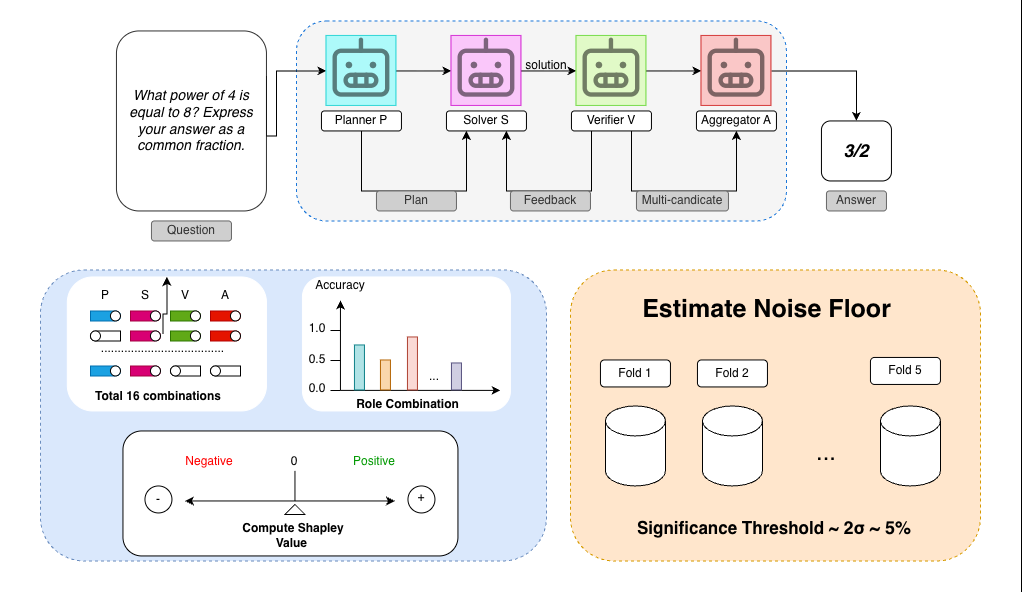
\includegraphics[width=0.9\linewidth]{figs/pipeline_shapley_overview.png}
\caption{The four-role pipeline, the 16 on/off coalitions that were run, and the 5-fold noise
estimation procedure.}
\label{fig:shapleyfw}
\end{figure}

\begin{table}[h]\centering\small
\begin{tabular}{@{}l c c@{}}
\toprule
Role & GSM8K 1.5B ($N=1319$) & MATH-500 1.5B ($N=500$)\\
\midrule
Planner    & $-0.0188$ $[-0.0399;+0.0021]$ & $+0.0210$ $[-0.0137;+0.0540]$\\
Verifier   & $+0.0555$ $[+0.0430;+0.0675]$ & $-0.0050$ $[-0.0257;+0.0150]$\\
Aggregator & $+0.0126$ $[+0.0052;+0.0202]$ & $+0.0040$ $[-0.0100;+0.0187]$\\
\bottomrule
\end{tabular}
\caption{Shapley values of the three roles with the solver held fixed, all roles at 1.5B. The
$\varphi$ values are on a 0--1 scale (the share of accuracy attributed to that role). By construction
the three values sum to the full pipeline's accuracy minus the solver's: $0.0493$ on GSM8K and
$0.0200$ on MATH-500. 95\% bootstrap CIs over questions --- \emph{no folds}, so read them together
with the noise floor in \S\ref{sec:setup}.}
\label{tab:shapley}
\end{table}

Table~\ref{tab:shapley} shows the following. On GSM8K, the verifier adds $0.0555$ and the aggregator $0.0126$, both with confidence intervals clear of zero, while the planner's value is negative with a confidence interval that reaches across zero. On MATH-500 none of the three intervals excludes zero, so on that benchmark none of the three roles can be separated from doing nothing. Either way the totals are small: the three roles together add 4.9 points on GSM8K and 2.0 points on MATH-500. The negative planner value on GSM8K is clearest in one pairwise comparison: $SA = 0.682 \to PSA = 0.562$, so adding the planner drops accuracy by 12 points.

Contributions also change with capability. On MATH-500, raising one role at a time to 7B while the others stay at 1.5B moves the planner from $+0.0210$ to $+0.0686$ (a change of $+0.0476$), the verifier from $-0.0050$ to $+0.1454$ (a change of $+0.1504$), and the aggregator from $+0.0040$ to $+0.1203$ (a change of $+0.1163$). The verifier shows the largest shift of the three: its contribution is not distinguishable from zero at 1.5B and becomes the largest of the three at 7B. This comparison is available on MATH-500 only; on GSM8K we ran the aggregator variant alone ($+0.0126 \to +0.1041$). The verifier result sets up \S\ref{sec:roles}.

One limitation matters for reading this table: Shapley assigns credit to the \emph{role label}, not to the \emph{function} performed --- if the planner quietly solves the problem, its work is still recorded under the label ``Planner'' even though the behaviour is the solver's. The next section analyses traces to ask whether the roles actually perform their assigned functions.

% ---------------------------------------------------------------
\subsection{The gap between the assigned role and the executed role}\label{sec:roles}

The verifier contributes nothing measurable at 1.5B and becomes the largest of the three contributors at 7B. That pattern is a reason to look at what the roles actually do, rather than at what they are called. Table~\ref{tab:behavior} collects behavioural measurements from traces, and shows that on small models role specialisation is mostly nominal: the planner --- despite being forbidden to compute the answer --- still contains the correct answer in 34.7\% of MATH problems (and in 45.3\% of cases also supplies the answer format); when a plan is present, the solver merely copies it (median solution length 19 characters, against 664 without a plan). On the 7B model these behaviours largely disappear --- but at that capability level the pipeline loses to the single solver. Across 2{,}000 turns over all four cells, the aggregator produced a new and correct answer only 3 times: the aggregation role does no computation at any capability level.

\begin{table}[h]\centering\small
\begin{tabular}{@{}l c c c c@{}}
\toprule
Behavioural measure (traces) & GSM8K 1.5B & MATH 1.5B & GSM8K 7B & MATH 7B\\
\midrule
Planner leaks the correct answer & 14.0\% & 34.7\% & 1.0\% & 4.0\%\\
Solver produces no new numbers & 60.7\% & 62.0\% & 1.0\% & 11.0\%\\
Solver solution length & 19 & 344 & 821 & 1247\\
Verifier intervenes & 32.7\% & 38.0\% & 4.0\% & 14.0\%\\
Aggregator repeats the verifier's answer & 93.3\% & 73.3\% & 100\% & 97.0\%\\
\bottomrule
\end{tabular}
\caption{Behaviour per cell (task $\times$ capability, $n=100--150$ per cell, measured on traces).}
\label{tab:behavior}
\end{table}

Two causal results support this table. \emph{First}: simply removing the line ``Do NOT compute the final answer'' from the planner's prompt \emph{raises} the downstream solver by $+3.8$ points on MATH and $+3.3$ on GSM8K --- the instruction only hides the answer, it does not stop the planner from computing it, and hiding it does harm. \emph{Second}, when prompts are permuted across positions, accuracy is indistinguishable: on GSM8K $0.660 = 0.660$ (the \texttt{solo} configuration reaches $0.673$); on MATH $\texttt{swap}-\texttt{normal} = +5.3$ points but $t=1.84$, CI $[-2.7;+13.4]$ --- not statistically significant. The wide CI does not let us rule out a medium-sized effect, so we record only that there is no evidence that ``role identity'' affects the outcome.

The checking role does not really check either. Three independent measurements: (i) when it intervenes, the 1.5B verifier is right only 56--59\% of the time --- close to chance; the 7B verifier is right 98\% of the time. (ii) An error-injection experiment --- altering the result of one computation step in a gold solution chain and then asking the model ``is there a calculation error?'' --- shows the 1.5B model answering ``no error'' on close to 100\% of problems, i.e. blind to the injected error; the 7B model passes the validity gate and separates clean from altered problems ($+0.651$ on the stratum of problems it can solve on its own; the stratum it \emph{cannot} solve on its own has only $n=9$, so the question of whether checking is separable from solving remains open). (iii) The \texttt{V\_gain} grid (Table~\ref{tab:vgaingrid}) shows that the checking turn pays off only within a narrow band.

\begin{table}[h]\centering\small
\begin{tabular}{@{}l c c@{}}
\toprule
\texttt{V\_gain} (points; min--max across folds) & GSM8K & MATH\\
\midrule
1.5B & $+4.4$ $[+1;+8]$, 5/5 positive & $+1.4$ $[-1;+4]$\\
7B   & $+1.0$ $[-3;+5]$ & $+4.4$ $[+2;+8]$, 5/5 positive\\
\bottomrule
\end{tabular}
\caption{\texttt{V\_gain} by task $\times$ capability (5 folds per cell). Ordering the four cells by
solver accuracy --- $0.402$ (overwhelmed); $0.598$ (pays off); $0.668$ (pays off); $0.884$
(saturated) --- the checking turn pays off only in the solver-accuracy band $\approx 0.60$--$0.67$:
below it the verifier is overwhelmed, above it there are no errors left to fix.}
\label{tab:vgaingrid}
\end{table}

The clearest driver is the capability of the model doing the checking. On the same 300 MATH problems (5 folds $\times$ 60), Table~\ref{tab:verifier} shows:

\begin{table}[h]\centering\small
\begin{tabular}{@{}l c c c@{}}
\toprule
Checking turn & Effect (points) & 95\% CI (points) & Repaired : Broken\\
\midrule
\textbf{Verifier 7B} (solver 1.5B) & $\mathbf{+14.0}$ & $[+7.4;\,+20.6]$ & $43:1$\\
Verifier 1.5B (same size) & $+3.0$ & CI contains 0 & $15:6$\\
Portion attributable to the larger model & $+11.0$ & $[+3.9;\,+18.1]$ & ---\\
\bottomrule
\end{tabular}
\caption{The asymmetric effect of capability at the checking turn on MATH. ``Repaired : Broken'' =
incorrect answers turned correct against correct answers turned incorrect; the same-size verifier
breaks 6 problems, while the 7B verifier breaks only 1 over the same 300 problems.}
\label{tab:verifier}
\end{table}

The mechanism from the traces: when the verifier intervenes, it reuses the solver's intermediate numbers at roughly one-fifth the rate it does when it agrees ($0.20$--$0.23$ against $0.96$). Intervening is therefore closer to re-solving than to step-by-step checking, and in effect the checking turn is equivalent to one extra generation. This fits the hypothesis that the $+14.0$ points come mainly from adding one generation from a stronger model. The same picture appears elsewhere: \texttt{V\_gain} is statistically significant on MATH 7B ($+4.4$ points; CI $[+1.5;+7.3]$) but not on MATH 1.5B ($+1.4$; $p=0.235$). A note for \S\ref{sec:protocols}: the verifier \emph{generates a new chain}, so it belongs to the repair class --- its measured $L$ is $1/300 \approx 0.003$, very small but structurally not zero.

The $+14.0$ figure is measured against the weak model. The next section applies the second and first controls together: comparison against a strong-model baseline, with token cost taken into account.

% ---------------------------------------------------------------
\subsection{The strong model alone remains the benchmark on both accuracy and cost}\label{sec:baseline}

\begin{table}[h]\centering\small
\begin{tabular}{@{}l c c c c@{}}
\toprule
Configuration & GSM8K & MATH & 7B tokens (GSM8K) & 7B tokens (MATH)\\
\midrule
S1.5B + V7B & 0.810 & 0.563 & 105k & 119k\\
\textbf{S7B alone} & \textbf{0.910} & 0.593 & 120k & 152k\\
S7B + V7B & 0.900 & \textbf{0.670} & 205k & 261k\\
\bottomrule
\end{tabular}
\caption{Comparison against the strong-model baseline: configurations that include a verification pass, measured against the strong model run alone (5 folds). The token columns count only tokens generated by the 7B model --- they cannot be compared directly across configurations built from different model sizes; the correction is given in Table~\ref{tab:flop}. The two middle columns are accuracy (0--1 scale), the last two are token counts (thousands).}
\label{tab:baseline}
\end{table}

Table~\ref{tab:baseline} moves the baseline from ``the weak model'' to ``the strong model alone'', and the picture changes. The asymmetric configuration S1.5B+V7B --- the same configuration that gave $+14.0$ points in Table~\ref{tab:verifier} --- is \emph{worse} than S7B alone by 10 points on GSM8K, and only matches it on MATH. The cost column needs two corrections: (a) the raw token column ignores the tokens spent by the 1.5B solver; (b) a 7B token costs roughly 4.7--4.9 times more than a 1.5B token in FLOPs. Table~\ref{tab:flop} rescales cost onto the FLOP axis:

\begin{table}[h]\centering\small
\begin{tabular}{@{}l c c@{}}
\toprule
Cost ratio (asymmetric / S7B) & Raw 7B tokens & FLOP-weighted\\
\midrule
GSM8K & $0.88\times$ (``12\% cheaper'') & $\mathbf{1.00\text{--}1.05\times}$ \\
MATH & $0.78\times$ (``22\% cheaper'') & $\mathbf{0.92\text{--}0.96\times}$ \\
\bottomrule
\end{tabular}
\caption{Correcting the unit price of a token (sensitivity swept over characters-per-token from 3.0 to 4.0). Prefill is not counted --- the 7B model has to \emph{read} the 1.5B solution --- so the correction still favours the asymmetric configuration.}
\label{tab:flop}
\end{table}

The conclusion: on GSM8K the asymmetric configuration is dominated outright (10 points worse, at equivalent FLOP cost); on MATH it saves a marginal 4--8\% at equivalent accuracy. The strong model alone sits on the Pareto frontier for both tasks.

The one bright spot in Table~\ref{tab:baseline} that is distinguishable from zero comes from the same-size configuration: adding V7B to S7B on MATH gives $+7.7$ points ($p=0.0075$; McNemar), at $1.7\times$ the token cost. In the notation of \S\ref{sec:identity} this is the case $\acc(E) > \acc(I)$ --- and it occurs at a \emph{capability gap of zero}. The same configuration on GSM8K spends $1.7\times$ the cost to lose 1 point --- the benefit of a same-size verification pass depends on the task. We return to this data point in \S\ref{sec:termG}, where it is the only evidence supporting the positive half of the capability-gap rule.

Because the same model pair on the same family of problems appears with several different values across this report, Table~\ref{tab:doichieu} lists them side by side to avoid confusion:

\begin{table}[h]\centering\small
\begin{tabular}{@{}l l l l l@{}}
\toprule
Value & Quantity & Baseline & Setup & Section\\
\midrule
$+14.0$ points & verification-pass effect & weak model (\texttt{PS}) & verification prompt, 300 problems & \S\ref{sec:roles}\\
$-3.0$ points & configuration accuracy & strong model (S7B) & as above, 5 folds & \S\ref{sec:baseline}\\
$-12.4$ points & $\dhonest = \acc(E)-\acc(I)$ & strong model & \emph{solve} prompt, artifact shown, $n=500$ & \S\ref{sec:termL}\\
$-16.6$ points & $\dceil$ (ideal ceiling) & strong model & repair prompt, bootstrap & \S\ref{sec:transfer}\\
\bottomrule
\end{tabular}
\caption{The same 1.5B$\to$7B pair on the maths domain, four different quantities. The change of sign between the first row and the three below it is the central phenomenon itself: changing the baseline changes the sign of the effect.}
\label{tab:doichieu}
\end{table}

One control is still missing: the denominator. Every number above is an average over the whole set --- including the problems that no mechanism could have rescued.

% ---------------------------------------------------------------
\subsection{Stratifying by the reach of the aggregation method}\label{sec:denominator}

\begin{table}[h]\centering\small
\begin{tabular}{@{}l c c c c@{}}
\toprule
Correct generations /5 & $n$ & Solver & maj@5 & $\Delta$ (points)\\
\midrule
0/5 --- too hard & 48 (32\%) & 0.000 & 0.000 & 0\\
1/5 & 20 (13\%) & 0.000 & 0.000 & 0\\
2/5 & 15 & 0.333 & 0.600 & $+26.7$\\
3/5 & 12 & 0.583 & 1.000 & $+41.7$\\
4/5 & 18 & 0.722 & 1.000 & $+27.8$\\
5/5 --- too easy & 37 (25\%) & 1.000 & 1.000 & 0\\
\bottomrule
\end{tabular}
\caption{Stratification by the number of correct generations out of 5 (MATH 1.5B, $n=150$). The $\Delta$ column is the accuracy difference between \texttt{maj@5} and the Solver.}
\label{tab:strata}
\end{table}

Table~\ref{tab:strata} splits the 150 problems by ``how many correct solutions the pool contains''. Two fixed quantities need to be kept apart. By the structure of the pool, 57\% of the problems (0/5 and 5/5) cannot show any effect under any aggregation method --- there is either nothing to select or nothing left to improve. For majority voting in particular, adding the 1/5 stratum (a single vote cannot win a majority) brings the total to 70\%. On the reachable strata, the effect of voting is $+21.5$ points (strata 1--4/5) or $+31.1$ points (strata 2--4/5); the full-set average dilutes this to $+9.3$ --- a dilution factor of 2.3--3.3 depending on how the strata are grouped. The strata are defined after the fact, using the generation results themselves, so this is an interpretive tool, not a deployable baseline. A genuine $+10$-point intervention that only reaches strata 2--4/5 (30\% of the problems) would show up as $+3.0$ points over the full set --- below the noise floor.

The three controls therefore pull in opposite directions: a missing denominator $\Rightarrow$ underestimate; a missing cost or baseline correction $\Rightarrow$ overestimate. Self-declared limitation: the headline effects in \S\ref{sec:roles}--\ref{sec:baseline} have not been re-stratified this way (we lack per-problem data for each stratum); their full-set numbers are therefore low estimates of the effect on the reachable strata.

\emph{End of the first thread.} The picture after three controls: the only value that is reliably positive is the extra generation; configurations in which models repair each other's work lose to the strong model alone. Act II asks where the value goes, and whether any rule predicts it in advance.

% ---------------------------------------------------------------
\subsection{The capability gap shrinks the opportunity for improvement}\label{sec:termG}

A raw observation over 7 model pairs, pooled across several runs: cross-family pairs have about 24\% more opportunity $G$ (0.0597 versus 0.0481), but cross-family pairs also have a smaller capability gap (0.130 versus 0.167); the two variables are completely confounded. A pre-registered design that separates them uses 6 models, 15 directed pairs, on the same 499 MBPP problems, with the regression
\begin{align*}
G &= \beta_0 + \beta_1\cdot\text{gap} + \beta_2\cdot\text{cross\_family}\\
\beta_1 &= -0.1922\ (p \approx 0)\\
\beta_2 &= +0.0045\ (\text{CI } [-0.0051;+0.0140];\ p = 0.31).
\end{align*}
The $R^2$ of the gap term alone is 0.824. The CI for $\beta_2$ lies entirely below the equivalence margin of $+0.02$ fixed in advance, which makes this an informative null: the cross-family effect is not separable from zero within that margin, and the explanatory variable is the capability gap. The sign of $\beta_1$ is worth reading carefully: the larger the gap, the smaller the opportunity $G$ --- the weaker the weak model, the fewer problems it can rescue for the strong one. (The pool-diversity result --- 3 models yield 2.70/3 distinct candidates versus 1.91/3 for a single model --- is recorded only as a different-model effect; the different-model, same-family control has not been run.)

Adding the repair branch for all 15 pairs (pre-registered) gives the rule for the ceiling:
\begin{equation}\label{eq:rule}
\dceil = +0.0218 - 0.2392 \times \text{gap};\qquad R^2 = 0.60;\ p = 10^{-5};\
g^\ast \approx 0.09,
\end{equation}
where $g^\ast = \beta_0/|\beta_1|$ is the gap at which the fitted line crosses zero (that is, $\approx 9$ accuracy points; we have not estimated a CI for $g^\ast$, so it describes a trend and is not yet an operational rule). Identity~\eqref{eq:identity} holds for 15/15 pairs. A mandatory caveat goes with this: 0/15 pairs are positive at the 5\% level and 3/15 are negative at the 5\% level --- on MBPP the rule can only be stated in its negative direction (once the gap exceeds $\sim$0.09, the repair protocol produces a negative effect); establishing the positive region would need about 8 times the MBPP data. Two data points outside MBPP probe the positive half: the 7B$\to$14B pair on MATH (gap $0.044 < g^\ast$) measures $-1.4$ points with a CI covering both signs, so it does not support the rule; the same-size configuration (gap $=0$) on MATH measures $+7.7$ points at the 5\% level (\S\ref{sec:baseline}), which does support it. The positive half therefore rests on ``one point in favour, one point inconclusive''. The gap explains 82\% of the variance in $G$ but only 35\% of the variance in $L$; most of the variation in the loss term comes from some other factor we have not identified (recorded under Limitations). (Mechanism note\mucB: the preservation threshold a repair pass has to clear grows with the gap twice as fast as its actual preservation ability --- coefficients 2.18 versus 1.10; $p=0.0066$ --- which suggests the negative effect arises from the structure of the $G$--$L$ budget rather than from any intrinsic degradation of the strong model.)

% ---------------------------------------------------------------
\subsection{Testing whether the capability-gap rule transfers to another domain}\label{sec:transfer}

We take the curve~\eqref{eq:rule} fitted on MBPP and use it to predict $\dceil$ on MATH (pre-registered; 3 Qwen pairs; paired bootstrap CI with 10\,000 resamples). The results are given in Table~\ref{tab:transfer}.

\begin{table}[htbp]
\centering
\small
\begin{tabular}{@{}l c c c c l@{}}
\toprule
Pair & Gap & Measured $\dceil$ & 95\% CI & MBPP prediction & Verdict\\
\midrule
7B$\to$14B & 0.044 & $-0.0140$ & $[-0.046;\,+0.018]$ & $+0.0108$ & inside the interval\\
1.5B$\to$7B & 0.244 & $-0.1660$ & $[-0.208;\,-0.124]$ & $-0.0361$ & outside the interval\\
1.5B$\to$14B & 0.288 & $-0.0680$ & $[-0.102;\,-0.034]$ & $-0.0471$ & inside the interval\\
\bottomrule
\end{tabular}
\caption{A test of whether the capability-gap relationship carries over to the maths domain. All values are on a 0--1 scale. The prediction column comes from a curve fitted on MBPP and applied to these problems without refitting.}
\label{tab:transfer}
\end{table}

Two of the three predictions fall inside the 95\% confidence interval, so the rule is not rejected. The intervals are wide, however (0.064--0.084), so the test has low resolution. Beyond that, the three points are not monotonic (a gap of 0.244 produces a deeper negative effect than a gap of 0.288), so monotonicity of the rule is not confirmed on the maths domain. The 1.5B$\to$7B pair falls outside in a systematic way, with $L = 0.166$, roughly 7 times $G$. The same behaviour reappears in an independent measurement on the same pair ($-0.1380 \to -0.1660$). The rule therefore describes a general trend only; the exceptions show up when the weak model is far too weak for the difficulty of the problems.
\subsection{The content of the artifact decides the effect of exposure}\label{sec:termL}

This is the central experiment of the study (pre-registered; we chose MATH-500 to change domain relative to the original exploratory observation on MBPP). The design is shown in Figure~\ref{fig:exposure}: the two branches $I$ and $E$ use the same solve instruction and are identical in every other respect, differing only in whether the context carries $W$'s artifact. Results are stratified by artifact content and reported in Table~\ref{tab:exposure}.

\begin{table}[htbp]
\centering
\small
\begin{tabular}{@{}l c c c@{}}
\toprule
Stratum & MBPP 11--510\mucB & MBPP 511--974\mucB & MATH-500 (level A)\\
\midrule
artifact wrong  & $-19.0$ & $-19.3$ & $-27.2$ ($p\approx 0$; $n=261$)\\
artifact correct & $+6.4$ & $+2.5$ & $+3.8$ ($p=0.012$; $n=239$)\\
\bottomrule
\end{tabular}
\caption{Exposure effect $\acc(E)-\acc(I)$ (units: percentage points), stratified by artifact content. The two MBPP columns are post hoc stratifications (level B); the MATH column is the pre-registered experiment (level A).}
\label{tab:exposure}
\end{table}

On the wrong-artifact stratum, the accuracy of the strong model drops from 46.4\% to 19.2\% --- on exactly the problems it was already solving nearly half the time. A correct artifact, by contrast, improves accuracy. Weighting the two strata reproduces $\dhonest = -12.4$ points. The mechanism follows: $D$ is not a penalty for seeing an artifact at all, but a penalty for seeing wrong content. Since the design carries no repair instruction, the mere presence of wrong content in the context is enough to produce the negative effect. (A matched control for the pure effect of context length has not been run; the closest control --- inserting irrelevant context in the checking setup\mucB{} --- gives $-3.6$ points, so pure context noise is mildly harmful, seven to eight times smaller than the wrong-content penalty.) This matches the low reuse rate under intervention in \S\ref{sec:roles}: the strong model rarely copies wrong content at the surface, yet is still anchored by it --- the influence travels through the choice of approach more than through quotation.

Table~\ref{tab:222} re-scores all 500 problems by the state pair ($W$ correct/wrong) $\times$ ($I$ correct/wrong), and records the share of correct $E$ answers in each cell, to answer whether repair helps when the strong model is wrong.

\begin{table}[htbp]
\centering
\small
\begin{tabular}{@{}l c c@{}}
\toprule
Stratum & $n$ & Share of $E$ correct (\%) \\
\midrule
$W$ correct, $I$ correct & 228 & 99.6\\
$W$ correct, $I$ wrong & 11 & 90.9\\
$W$ wrong, $I$ correct (risk zone) & 121 & 36.4 \quad (destroys 63.6\%)\\
Both wrong & 140 & 4.3\\
\bottomrule
\end{tabular}
\caption{$2\times 2$ stratification by the states of $W$ and $I$ on MATH ($n=500$), with the share of correct $E$ answers in each stratum.}
\label{tab:222}
\end{table}

Three main observations follow from Table~\ref{tab:222}. First, the repair protocol acts as a conduit, not an error corrector: it almost never produces a new solution when both models miss (4.3\% = 6/140), it destroys at scale in the risk zone (63.6\% = 77/121), and it passes through $W$'s correct answer when there is one (10 of 11 problems --- the stratum is too small for a tight estimate). Second, for this pair the exploitable stratum is 11 times smaller than the risk zone (11 problems against 121); that ratio scales with the capability gap, but we did not measure it at other gap sizes. Third, the strategy ``keep $W$ when $W$ is right'' is equivalent to the $\CEIL$ oracle. Even when handed that oracle, the gain is only $+0.4$ points (2 more correct out of 500), because $E$ already retains 99.6\% and 90.9\% in the two corresponding strata. Even at $\CEIL = 0.578$, the value stays below $I = 0.698$. Within the class of asymmetric repair protocols we measured, no configuration reached $\acc(E) > \acc(I)$ (0/15 MBPP pairs, best $-3.0$ points; the MATH pairs are in Table~\ref{tab:transfer}); the only case of $E>I$ is the same-size configuration in \S\ref{sec:baseline}. The problem is not that the system ``forgets to keep $W$'', it is that $E$ destroys the risk zone. Among the options we tried (the two oracle gates in \S\ref{sec:kappa}), only keeping the artifact out of the context protected that zone.

\subsection{From verification signal to selection and routing}\label{sec:kappa}

\paragraph{A certain signal.}
On HumanEval, with the same model and the same 4 generations, differing only in the source of the check, the results are in Table~\ref{tab:exec}.

\begin{table}[htbp]
\centering
\small
\begin{tabular}{@{}l c c c c c@{}}
\toprule
Condition & greedy & exec3 & llm3 & exec3 destroyed & llm3 destroyed\\
\midrule
HE 1.5B (run 1)  & 0.5375 & 0.6000 & 0.4812 & 0.0 & 2.8\\
HE 1.5B (run 2)    & 0.5625 & 0.6438 & 0.4375 & 0.0 & 4.6\\
HE 7B (run 1)      & 0.8000 & 0.8812 & 0.7812 & 0.0 & 2.6\\
HE 7B (run 2)   & 0.7938 & 0.9000 & 0.7438 & 0.0 & 3.2\\
\bottomrule
\end{tabular}
\caption{Selection by running tests (\texttt{exec3}) compared with LLM self-review (\texttt{llm3}). Each model was measured twice; the two runs per model were collected on two different hardware setups, but the table does not record which run corresponds to which setup. The spread between the two runs of a model is about 0.03, smaller than the effect of interest, so the conclusions about sign still hold. The ``destroyed'' columns give the number of problems broken per fold. }
\label{tab:exec}
\end{table}

exec3 destroyed nothing in 20 of 20 folds and matched \texttt{oracle@4} exactly in the two cells where that figure was recorded (0.6438 and 0.8812). llm3, by contrast, destroyed solutions in all 20 folds. The honest baseline is greedy; majority voting is harmful on code, because long solutions rarely coincide verbatim. The difference $exec3-\text{greedy}$ ranges from $+6.3$ to $+10.6$ points across the four conditions. One condition on the application side matters: when the base model is saturated (GSM8K 7B, solver 0.916), an execution checker with accuracy 0.837 still gives a net negative effect (26 destroyed / 6 fixed). ``Having a certain checker'' is therefore only worth something while headroom remains.

\paragraph{A learned signal.}
The classifier was trained on injected errors (take a correct solution and change one digit in the answer) and then used to detect real errors. This is also the test ``change one number in the answer --- does the verifier notice?''. Results are in Table~\ref{tab:clf}.

\begin{table}[htbp]
\centering
\small
\begin{tabular}{@{}l c c c c@{}}
\toprule
Model & Separation on injected errors & Separation on real errors & AUC & $\Delta$ accuracy\\
\midrule
1.5B & $-0.012$ & $+0.195$ & 0.528 & $-0.8$ points (1/5 folds positive)\\
\textbf{7B} & $\mathbf{+0.573}$ & $\mathbf{+0.693}$ & \textbf{0.893} & $\mathbf{+2.4}$ points (2/5 folds positive)\\
\bottomrule
\end{tabular}
\caption{Effectiveness of the learned error classifier. The first two columns give the separation in
classifier score between correct and wrong solutions, measured on injected and on real errors. At 1.5B, AUC $0.528 \approx$ random guessing: change one digit in the
answer and the 1.5B verifier does not detect it.}
\label{tab:clf}
\end{table}

At 7B the measured signal is good (AUC = 0.893; separation is even better on real errors than on injected ones, so we would need to rule out the classifier latching onto surface features such as length; that control has not been run). But when the signal is used for selection, the improvement is only $+2.4$ points, and only 2 of 5 folds are positive. By our own sign test, this gain is not distinguishable from 0. A measurable signal therefore does not automatically become a usable one, which supports the upper-bound statement below.

\paragraph{A combined statement.}
Placed side by side: on code the $\texttt{oracle@}k-\texttt{maj@}k$ gap is wide and exec3 takes nearly all of it (it matches \texttt{oracle@4} exactly and destroys nothing); on math the gap is 12--13 points (Table~\ref{tab:budget}) but the best learned signal takes only $+2.4$ points.

\begin{quote}
The gap $\texttt{oracle@}k - \texttt{maj@}k$ is an upper bound on the value of any checker over the same pool. A certain signal (running tests) takes nearly all of that bound; the learned signal in our study takes only a small part of it, even though its error measurement is of high quality. The bottleneck in the math domain is therefore twofold: no certain signal, and a poor pool. Among the problems where \texttt{maj@5} is wrong, 65\% (48/74, computed from Table~\ref{tab:strata}) are problems whose pool does not contain a single correct candidate, so no selector could rescue them.
\end{quote}

\paragraph{Routing.}
Both results on ``choosing when an extra call is needed'' are level B (measured once, $n=300$). The consensus router (run $S$ and $V$, call $A$ only when the two roles disagree) on GSM8K keeps almost all of the pipeline's benefit at 77\% of the cost (0.720 against 0.723, at 2.32 against 3 calls); on MATH it reaches 0.413, equal to the solver alone and therefore of no benefit. The mechanism behind this is consistent with \S\ref{sec:termL}: the share of problems the weak model gets wrong (that is, the share of wrong artifacts in the context) is about 33\% on GSM8K against 59\% on MATH; when the two roles disagree, $A$ rescues 45.4\% of cases on GSM8K but only 25.0\% on MATH. The observation that ``routing saves cost exactly where saving is least needed'' therefore stays at level B.

Two ceilings for the exposure gate (computed on the data of \S\ref{sec:termL}): a perfect artifact gate (show only correct artifacts --- an oracle) reaches $+1.8$ points over $I$; a real classifier would need about 88--89\% accuracy to break even (break-even $\approx 27.2/(27.2+3.8)$ from the two effects in Table~\ref{tab:exposure}). A gate that knows when $I$ is wrong (a stronger oracle) reaches $+3.2$ points, but it requires detecting the strong model's own errors --- exactly the kind of signal we have just shown to be measurable but not usable. The implication is that improving the gate has a low ceiling; the default configuration, which keeps the artifact out of the context, has a higher expected value.

\subsection{Role training and the shortcuts of the objective function}\label{sec:rl}

\begin{figure}[h]
\centering
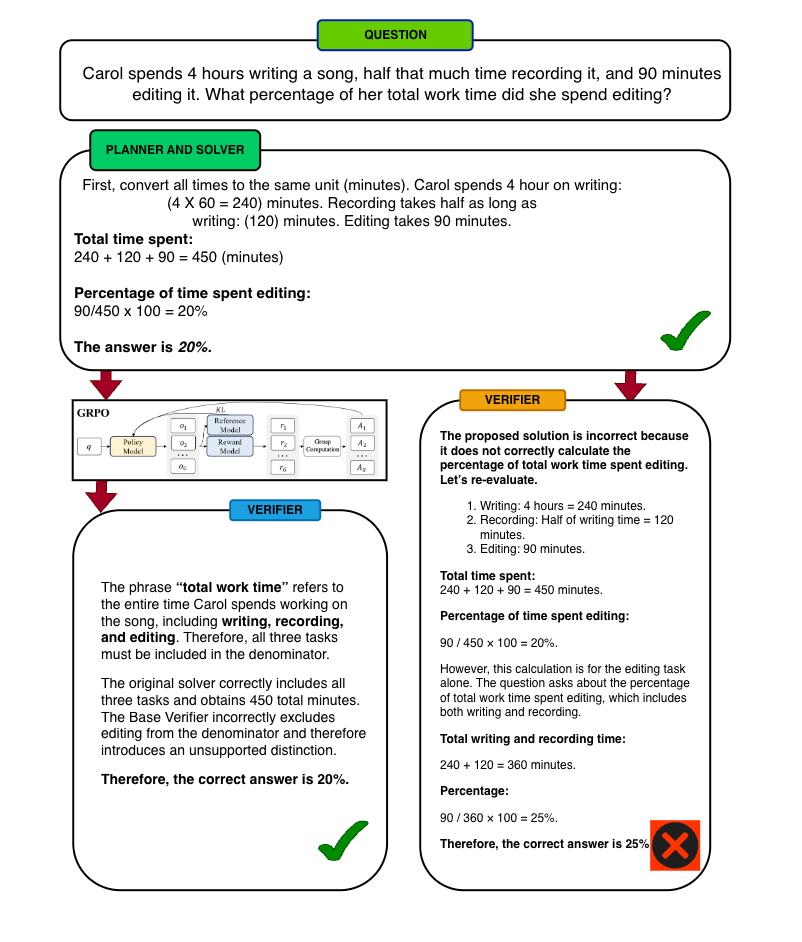
\includegraphics[width=0.65\linewidth]{figs/verifier_grpo_example.png}
\caption{A concrete case on GSM8K: the solver answers correctly (20\%), the original verifier ``fixes'' it into a wrong answer (25\%) --- exactly the risk-zone destruction of \S\ref{sec:termL}; the verifier after GRPO keeps the correct answer, but it achieves that mainly by intervening less, not by checking better. Figure reused from the group's Shapley block report.}
\label{fig:grpoexample}
\end{figure}

We tried seven methods for training and optimising roles. None met the project standard (effect above threshold and 5/5 folds with the same sign) on held-out data, and every failure traced back to the model finding a shortcut in the objective function instead of learning the target skill.

\begin{description}\itemsep5pt
\setlength{\leftmargini}{1.6em}\setlength{\labelsep}{0.5em}
\item[\textbf{First.}] GRPO verifier with reward $+1$ for a correct fix, $-1$ for a destruction, $0$ for silence. After training, precision rises from $0.70$--$0.90$ to $1.00$ (5/5 folds), but \texttt{V\_gain} falls from $+6.8$ to $+4.4$ points, and the number of interventions falls from $20.2$ to $8.4$ per 100 problems. The shortcut is ``free silence'': perfect precision is obtained by the model speaking half as often.


\item[\textbf{Second.}] GRPO on the final answer (patching the silence hole) reaches $+1.8$ points, below the $+2.0$ threshold fixed in advance. The shortcut is mimicking the solver: median output length falls from $480$ to $19$ characters, and the rate of agreeing when the solver is wrong rises from $0.50$ to $0.64$.

\item[\textbf{Third.}] GRPO with information asymmetry (solver 0.5B, verifier 1.5B; pre-registered, with a full $I$ branch) measures two baselines at once: against the weak model it gives $+17.0$ points (5/5 folds positive); against the checking model itself solving on its own it gives $-10.4$ points (5/5 folds negative). RL recovers only 38\% of the exposure damage; 54\% of the broken problems produce a third answer that follows neither model.

\item[\textbf{Fourth.}] ORPO aggregator (learning from preference pairs) reaches $+3.3$ points on MATH (3/5 folds, below the noise floor) and $-2.7$ points on GSM8K cross-task. The shortcut is amplifying the habit of copying the last candidate (from $0.71$ to $0.81$) and learning to ``solve it again'' instead of to select.

\item[\textbf{Fifth.}] Credit-RL (rewarding roles by their marginal Shapley contribution) improves no role by the 5/5-fold standard. The planner collapses to empty plans on 200 of 200 problems; the verifier makes 23 fixes and 24 destructions.

\item[\textbf{Sixth.}] Credit-RL stage 2 (a shortcut-resistant design) gives V-COND $+3.0$ points (4/5 folds positive) on GSM8K, the only positive variant, but it does not carry across domains: on MATH it gives $-7.0$ points (5/5 folds negative).

\item[\textbf{Seventh.}] MAPoRL co-training of S/V/A leaves the result unchanged ($0.690 \to 0.690$), because the aggregator was bottlenecked throughout training.
\end{description}

Each method had either a design fixed in advance or an effect gate; per-run details and
corrections are in \texttt{docs/}. The eighth method --- the supervised classifier
--- was presented in Table~\ref{tab:clf}.

\looseness=-1
Figure~\ref{fig:grpoexample} illustrates one concrete case. The information-asymmetry experiment (method three) is the one worth singling out, because it measured two baselines on the same run. Against the weak model, the effect is $+17.0$ points (5/5 folds positive); against the checking model itself when it does not see the artifact, the effect is $-10.4$ points (5/5 folds negative). This is a training-based replication of the sign flip under a change of baseline (\S\ref{sec:synthesis}): RL narrows the exposure damage (recovering 38\%) but does not reverse the sign of $\dhonest$. The general conclusion across all these methods connects straight to \S\ref{sec:kappa}: when the reward signal is itself only a learned signal, optimisation finds the shortcut in that signal faster than it finds real checking ability.
\section{Synthesis: the choice of baseline sets the sign of the effect}\label{sec:synthesis}

The two observations above point in opposite directions at first reading. \S\ref{sec:roles} records a
large capability gap together with a gain of $+14.0$ points, while \S\ref{sec:termG} shows that a large
gap drives the maximum attainable improvement $\dceil$ negative.

They do not conflict. They are two measurements against two different baselines, and the capability gap
moves the two baselines in opposite directions (Figure~\ref{fig:twobaselines}):
\begin{itemize}\itemsep2pt
\item \emph{Measured against the weak model $W$} (the baseline most studies report against): the
      checking role amounts to one more independent solution attempt by a stronger model
      (\S\ref{sec:roles}). What the number reflects is the intrinsic capability difference plus the
      advantage of an extra generation, so the gain grows with the capability gap (from $+3.0$ points
      at a gap of 0 to $+14.0$ points at a gap of 0.244).
\item \emph{Measured against the strong model run independently $I$} (the baseline that matters in
      deployment): the net value follows $G - L + R$. The improvement opportunity $G$ shrinks as the
      gap widens ($\beta_1 = -0.19$, \S\ref{sec:termG}), while the loss $L$ grows (on MATH at a gap of
      0.244, $L$ is about 7 times $G$ in magnitude). The combined value therefore falls, and the only
      positive configuration appears when the two models are of comparable capability ($+7.7$ points at
      a gap of 0, \S\ref{sec:baseline}).
\end{itemize}
What we are seeing is not a property of the coordination mechanism but of the baseline we choose to
compare against. A capability gap inflates the apparent effect relative to the weak model and erodes
the real added value relative to the strong model. The exposure-loss mechanism (\S\ref{sec:termL})
accounts for the erosion: the wider the capability gap, the more likely the artifact is wrong, and the
more often the strong model is steered off a problem it could have solved on its own.

\begin{figure}[!ht]\centering
\begin{tikzpicture}[x=255mm, y=1.85mm]
  % 1. Vung nen phan chia
  \fill[blue!5, rounded corners=3pt] (0, 0) rectangle (0.091, 16.5);
  \fill[red!4, rounded corners=3pt] (0.091, -18.5) rectangle (0.32, 0);

  % 2. Luoi toa do nhe
  \draw[help lines, color=gray!25, xstep=0.05, ystep=5] (0, -18.5) grid (0.32, 16.5);

  % 3. Truc toa do
  \draw[->, >=Stealth, thick, black!80] (-0.012, 0) -- (0.335, 0) node[right=4pt, font=\footnotesize\bfseries] {Capability gap};
  \draw[->, >=Stealth, thick, black!80] (0, -19.5) -- (0, 18.5) node[above=4pt, font=\footnotesize\bfseries] {Net effect (points)};

  % 4. Ticks tren truc
  \foreach \x/\l in {0.05/0.05, 0.1/0.10, 0.15/0.15, 0.2/0.20, 0.25/0.25, 0.3/0.30}
    \draw[thick, black!75] (\x, 0.6) -- (\x, -0.6) node[below=3pt, font=\footnotesize] {$\l$};
  \foreach \y in {-15, -10, -5, 5, 10, 15}
    \draw[thick, black!75] (0.002, \y) -- (-0.002, \y) node[left=3pt, font=\footnotesize] {$\y$};
  \node[below left=2pt, font=\footnotesize] at (0,0) {$0$};

  % 5. Nguong doi dau g*
  \draw[dashed, thick, gray!80!black] (0.091, -18.5) -- (0.091, 16.5);
  \node[draw=gray!50, fill=white, rounded corners=2pt, font=\scriptsize\bfseries, inner sep=2.5pt] at (0.091, 17.5) {Threshold $g^\ast \approx 0.09$};

  % 6. Duong xanh: So voi mo hinh yeu (MATH)
  \draw[very thick, blue!80!black] (0, 3.0) -- (0.244, 14.0);
  \fill[blue!80!black] (0, 3.0) circle (2.2pt);
  \node[above right=1pt, blue!90!black, font=\footnotesize\bfseries] at (0, 3.0) {$+3.0$};
  \fill[blue!80!black] (0.244, 14.0) circle (2.2pt);
  \node[above=2pt, blue!90!black, font=\footnotesize\bfseries] at (0.244, 14.0) {$+14.0$};

  % 7. Duong do: Tran Delta_tran so voi mo hinh manh (MBPP)
  \draw[very thick, red!75!black, dashed] (0, 2.18) -- (0.32, -5.47);

  % 8. Diem do thuc nghiem MATH
  \fill[red!75!black] (0.044, -1.4) circle (2.2pt);
  \node[left=3pt, font=\scriptsize\bfseries, red!85!black] at (0.044, -1.4) {$-1.4$};

  \fill[red!75!black] (0.244, -16.6) circle (2.2pt);
  \node[below=2pt, font=\footnotesize\bfseries, red!85!black] at (0.244, -16.6) {$-16.6$};

  \fill[red!75!black] (0.288, -6.8) circle (2.2pt);
  \node[below right=-1pt, font=\scriptsize\bfseries, red!85!black] at (0.288, -6.8) {$-6.8$};

  % 9. Diem cung quy mo tai chenh = 0
  \node[draw=red!75!black, fill=white, line width=1.1pt, inner sep=2.2pt] at (0, 7.7) {};
  \node[above right=1pt, font=\footnotesize\bfseries, red!85!black] at (0, 7.7) {$+7.7$};

  % 10. Nhan chu thich vung
  \node[font=\scriptsize\itshape, text=blue!80!black, anchor=north west] at (0.004, 15.2) {Ceiling region $\dceil > 0$ (headroom remains)};
  \node[font=\scriptsize\itshape, text=red!70!black, anchor=center] at (0.165, -10.5) {Ceiling region $\dceil < 0$ (net loss)};

  % 11. Hop Legend nam phia duoi do thi
  \node[draw=gray!45, fill=white, fill opacity=0.98, text opacity=1, rounded corners=3pt, font=\scriptsize, anchor=north, align=center, inner sep=4pt] at (0.16, -22.5) {
    \tikz[baseline=-0.5ex]{\draw[very thick, blue!80!black] (0,0) -- (0.35cm,0); \fill[blue!80!black] (0.175cm,0) circle (1.8pt);} Against the \emph{weak model} $W$ (MATH) \qquad\qquad
    \tikz[baseline=-0.5ex]{\draw[very thick, red!75!black, dashed] (0,0) -- (0.35cm,0);} Ceiling $\dceil$ against the \emph{strong model} $I$ (MBPP fit) \\[2pt]
    \tikz[baseline=-0.5ex]{\fill[red!75!black] (0.175cm,0) circle (2pt);} Measured $\dceil$ on MATH (Table~\ref{tab:transfer}) \qquad
    \tikz[baseline=-0.5ex]{\node[draw=red!75!black, fill=white, inner sep=1.4pt] at (0.175cm,0) {};} Same-size control ($\text{gap}=0$)
  };
\end{tikzpicture}
\caption{Two baselines, two directions of change. The horizontal axis is the capability gap. The effect
measured against the \emph{weak model} $W$ (solid blue line) rises with the gap; the ceiling on net value
$\dceil$ against the \emph{strong model} $I$ (dashed red line: fit over 15 MBPP pairs; red dots: 3 MATH
measurements) falls quickly and turns negative past the critical threshold $g^\ast \approx 0.09$, where
the exposure loss $L$ outweighs the improvement opportunity $G$.}
\label{fig:twobaselines}
\end{figure}

Five experimental results and one structural consequence support this reading: (1) \emph{structurally},
the selection protocol removes the loss entirely ($L=0$) by construction --- this follows from how the
protocol is defined and is not a measurement; (2) \emph{in magnitude}, the loss $L$ outweighs the
improvement opportunity $G$ ($L \approx 7G$) at a large capability gap on MATH --- in the 2$\times$2
stratified table (Table~\ref{tab:222}) $L$ covers 77 of the 500 problems against 11 for $G$. This ratio
between the two terms is a different quantity from the stratum-size ratio reported in the same table,
where the exploitable stratum is 11 times smaller than the at-risk stratum (11 problems against 121);
the two share the numeral 11 but are not the same comparison; (3) \emph{mechanistically}, the loss comes
directly from exposure to a wrong artifact, which we confirmed in a pre-registered experiment on two task
domains; (4) \emph{at the theoretical ceiling}, even ideal routing yields only a modest $+1.8$ points
against a decline of $-12.4$ points; (5) \emph{on generality}, the rule established on MBPP holds on 2 of
the 3 model pairs in the MATH set; and (6) \emph{on reproducibility through training}, reinforcement
learning under information asymmetry records a gain of $+17.0$ points against the weak model and a drop of
$-10.4$ points against the strong model at the same time, on 5 of 5 folds (\S\ref{sec:rl}). Independent
reports that multi-agent debate underperforms self-consistency on small models \cite{chen2025debate} point
in the same direction.

\paragraph{System design recommendations} (for the 1.5B--32B range on reasoning tasks). Three conditions
decide whether a multi-agent arrangement is worth building; failing any one of them leads to the same
recommendation, which is to use the strong model alone:
\begin{itemize}\itemsep2pt
\item \textbf{Domains with a deterministic verification signal} \emph{where the model has not saturated}:
      the best option is to generate candidates independently and select on execution results. This
      approaches the oracle ceiling without damaging solutions that were already correct. Once the base
      model has saturated on accuracy, adding a checker can lower overall performance (we recorded 26
      cases broken against 6 cases fixed on GSM8K 7B).
\item \textbf{Domains without a deterministic verification signal}: majority voting captures most of the
      available headroom on small models (43\% on MATH 1.5B), but the effect drops on larger models (8\%
      on 7B) and can backfire on code generation. An LLM aggregation role gives no consistent advantage
      over mechanical voting. Learned classification signals separate well on the held-out set but have
      not improved end-task accuracy.
\item \textbf{Cross-model coordination}: handing a small model's artifact to a large model for repair
      gives a negative effect or one that is not distinguishable from zero, particularly once the
      capability gap exceeds $\sim$0.09 (on MBPP). The checker has to be stronger than what it checks,
      and here it is the checked artifact that drags the checker down. In this case the option that is
      best on both accuracy and cost is to call the strong model alone.
\end{itemize}
Even when all three conditions hold, an unverified solution from a weak model should not be placed in a
strong model's context.

% =====================================================================
\section{Conclusion and limitations}\label{sec:limits}

The practical value of multi-agent LLM systems does not reduce to a single verdict. It depends
systematically on three measurable quantities: (1) the improvement opportunity $G$, which is set by
the capability gap and tends to narrow as that gap widens; (2) the exploitability $\kappa$, which
depends on whether the verification signal is deterministic rather than on the estimated quality of
the classifier; and (3) the exposure loss $L$, which arises from contact with a wrong artifact, and
where repair protocols act mainly as a conduit for the answer rather than as a genuine fix to the
reasoning (\S\ref{sec:termL}). The capability gap between models both raises the apparent
improvement relative to the weak model $W$ and erodes the net value relative to the strong model
$I$. In domains with a deterministic verification mechanism, multi-agent coordination approaches
the oracle ceiling without damaging solutions that were already correct --- but this holds only
while the base model is unsaturated; a strong checker applied to a saturated model still nets
negative. In open-ended reasoning domains, by contrast, the most effective architecture is
independent sampling followed by mechanical aggregation, keeping intermediate artifacts out of the
context of downstream models. Finally, many results that looked promising at first no longer
reached statistical significance once three strict controls and a pre-registered procedure were
applied together (16 of 32 runs were invalidated). That is an argument for experimental discipline when evaluating language-agent
systems.

\paragraph{Limitations.}
\begin{enumerate}\itemsep2pt
\item \textbf{Coverage of the deployable quantity $\dhonest$}: the experimental space of $\dhonest$
      has so far been surveyed on 15 directed model pairs on MBPP (0/15 of them reached a positive
      value that was statistically significant), one asymmetric pair on MATH ($-12.4$ points), and
      one same-capability configuration ($+7.7$ points). Three extended cross-checks did not finish
      because of the 14.6 GB VRAM limit of the free GPU: 8/9 generation branches are complete, and
      one branch remains --- its result has not been read.
\item \textbf{Variability of the \texttt{A\_gain} metric}: after standardising the \verb|\boxed|
      output format, two independent runs recorded improvements of $+0.8$ and $+8.0$ points
      respectively. Both are non-negative, but the difference in magnitude (which comes from
      different data partitions and different model quantisation levels) means the claim that the
      aggregation role is neutral still needs confirmation at larger scale.
\item \textbf{How much variance in the loss $L$ is explained}: the capability gap explains 82\% of
      the variance in the improvement opportunity $G$, but only 35\% of the variance in the exposure
      loss $L$. Most of the variation in $L$ therefore still comes from architectural or protocol
      factors that we have not modelled fully.
\item \textbf{Statistical sensitivity of some control groups}: the role-permutation test on MATH has
      a relatively wide confidence interval (upper bound $+13.4$ points). Several in-depth control
      conditions have not been run in full, including an extra generation without the artifact, a
      context-length control under the exposure condition, and a comparison between different models
      within the same architecture family. In addition, the Shapley analysis (\S\ref{sec:shapley})
      currently rests on bootstrap over problem samples and has not been analysed over independent
      data folds.
\item \textbf{Cross-domain generalisation}: the analysis transferring the pattern to the
      mathematics domain rests on only 3 model pairs with wide confidence intervals; the positive
      region of the capability-gap regression currently has a single empirical point ($+7.7$ points
      at a gap of zero) and does not have the statistical sensitivity to be established firmly on
      MBPP; the sign-change threshold $g^\ast$ has no parametric confidence interval attached.
\item \textbf{Decoding strategy and denominator stratification}: the information-flow branch of the
      study mainly uses a deterministic decoding strategy (greedy decoding), so each configuration
      has a single point estimate; the main effects have not been stratified exhaustively over the
      subset of problems where an effect is possible.
\item \textbf{Range of model scales}: every empirical conclusion in this study was established on
      models from 1.5B to 32B parameters on structured reasoning tasks, so it cannot be extended
      directly to very large language models ($>70$B); the training results (\S\ref{sec:rl}) in
      particular were all run on 0.5--1.5B models. The two evaluation standards we used (5-fold
      error bars and a pre-registration lock) also need more thorough cross-validation in follow-up
      work.
\end{enumerate}


% =====================================================================
\clearpage
\section*{Member contributions}

\newenvironment{ddgop}%
  {\begin{list}{$\bullet$}{%
     \setlength{\leftmargin}{1.4em}\setlength{\labelwidth}{0.8em}%
     \setlength{\itemsep}{1pt}\setlength{\parsep}{0pt}\setlength{\topsep}{3pt}}}%
  {\end{list}}

\paragraph{Dương Trọng Nguyên.}
\begin{ddgop}
\item Checking whether the roles actually perform the function they were assigned
\item Designing and running the artifact-exposure experiment
\item Calibrating the noise floor and controlling the denominator
\item Report: abstract, measurement methods, experimental setup; terminology consistency throughout
\end{ddgop}

\paragraph{Trương Đình Đức.}
\begin{ddgop}
\item Seven role-training methods and the shortcut analysis for each of them
\item Directions tried and dropped: backward reasoning, solve-then-grade, problem decomposition,
few-shot prompting for roles
\item Writing the analysis notes for the experiments
\item Report: introduction, related work, bibliography
\end{ddgop}

\paragraph{Trần Tùng Dương.}
\begin{ddgop}
\item Experiment infrastructure on Kaggle and the results-collection system
\item Scoring toolkit for the benchmarks
\item Measuring exploitability, training the error classifier, routing experiments
\item Report: synthesis, conclusion and limitations; presentation slides
\end{ddgop}

\paragraph{Lê Hoàng Quân.}
\begin{ddgop}
\item Measuring role contributions with Shapley values and interaction indices
\item Controlling the generation budget and the baselines
\item The capability-gap pattern and the cross-domain check
\item Report: results section; statistics toolkit
\end{ddgop}

% =====================================================================
\begin{thebibliography}{99}\small
\bibitem{austin2021} J. Austin et al. \emph{Program Synthesis with Large Language Models.}
arXiv:2108.07732, 2021.
\bibitem{bh1995} Y. Benjamini, Y. Hochberg. \emph{Controlling the False Discovery Rate.}
JRSS--B 57(1), 1995.
\bibitem{chen2021} M. Chen et al. \emph{Evaluating Large Language Models Trained on Code.}
arXiv:2107.03374, 2021.
\bibitem{chen2025debate} Y. Chen et al. \emph{When and Why Does Multi-Agent Debate Fail and Does It
Really Underperform?} arXiv:2510.20963, 2025.
\bibitem{cobbe2021} K. Cobbe et al. \emph{Training Verifiers to Solve Math Word Problems.}
arXiv:2110.14168, 2021.
\bibitem{du2024} Y. Du et al. \emph{Improving Factuality and Reasoning in Language Models
through Multiagent Debate.} ICML, 2024.
\bibitem{gou2024} Z. Gou et al. \emph{CRITIC: Large Language Models Can Self-Correct with
Tool-Interactive Critiquing.} ICLR, 2024.
\bibitem{grattafiori2024} A. Grattafiori et al. \emph{The Llama 3 Herd of Models.}
arXiv:2407.21783, 2024.
\bibitem{guo2024} D. Guo et al. \emph{DeepSeek-Coder: When the Large Language Model Meets
Programming.} arXiv:2401.14196, 2024.
\bibitem{hendrycks2021} D. Hendrycks et al. \emph{Measuring Mathematical Problem Solving with
the MATH Dataset.} NeurIPS, 2021.
\bibitem{huang2024} J. Huang et al. \emph{Large Language Models Cannot Self-Correct Reasoning
Yet.} ICLR, 2024.
\bibitem{kaplan2020} J. Kaplan et al. \emph{Scaling Laws for Neural Language Models.}
arXiv:2001.08361, 2020.
\bibitem{lightman2024} H. Lightman et al. \emph{Let's Verify Step by Step.} ICLR, 2024.
\bibitem{madaan2023} A. Madaan et al. \emph{Self-Refine: Iterative Refinement with
Self-Feedback.} NeurIPS, 2023.
\bibitem{mad2025baseline} \emph{Multi-LLM-Agents Debate --- Performance, Efficiency, and Scaling
Challenges.} ICLR Blogposts, 2025.
\bibitem{masprm2025} \emph{MASPRM: Multi-Agent System Process Reward Model.} arXiv:2510.24803,
2025.
\bibitem{sharp2025} \emph{SHARP: Shapley Credit-based Optimization for Multi-Agent System.}
arXiv:2602.08335, 2026.
\bibitem{shapley1953} L. S. Shapley. \emph{A Value for $n$-Person Games.} Contributions to the
Theory of Games II, 1953.
\bibitem{shinn2023} N. Shinn et al. \emph{Reflexion: Language Agents with Verbal Reinforcement
Learning.} NeurIPS, 2023.
\bibitem{snell2024} C. Snell et al. \emph{Scaling LLM Test-Time Compute Optimally Can Be More
Effective than Scaling Model Parameters.} arXiv:2408.03314, 2024.
\bibitem{wang2023} X. Wang et al. \emph{Self-Consistency Improves Chain of Thought Reasoning in
Language Models.} ICLR, 2023.
\bibitem{wei2022} J. Wei et al. \emph{Chain-of-Thought Prompting Elicits Reasoning in Large
Language Models.} NeurIPS, 2022.
\bibitem{yang2024} A. Yang et al. \emph{Qwen2.5 Technical Report.} arXiv:2412.15115, 2024.
\bibitem{zheng2023} L. Zheng et al. \emph{Judging LLM-as-a-Judge with MT-Bench and Chatbot
Arena.} NeurIPS, 2023.
\end{thebibliography}

% =====================================================================
\appendix
\section*{Code and data}
All source code, summary results and experiment logs are published at\\
\url{https://github.com/duongtrongnguyen123/multiagent-shapley-credit}\\
(branch \texttt{archive}; the \texttt{main} branch contains only the report and the slides).

\end{document}
